\subsection{Was ist ein geswitchtes Netz?}
\label{sec:geswitchtes_netz}
Ein geswitchtes Netzwerk zeichnet aus, dass die Auslastung des Netzwerke durch den Datenfluss der Netzwerkteilnehmer stark reduziert wird, da ein Frame nur an die Ziel-Adresse gesendet wird, wenn sie bereits in der Switch-Tabelle hinterlegt ist.

Somit bringt der Einsatz eines Switches auch mehr Sicherheit, wenn es darum geht, wer im Netzwerk hängt und wer welche Daten erhalten soll.

Ein Switch kann Netzwerkteilnehmer auch in Gruppen aufspalten und hier unterscheiden, an welche Gruppe das Frame zugestellt werden soll, das Verhalten ist wie bei zwei getrennten LAN.
Die Netzwerkteilnehmer sehen dann nur die Frames in ihrer Gruppe.

\begin{figure}[H]
	\centering
	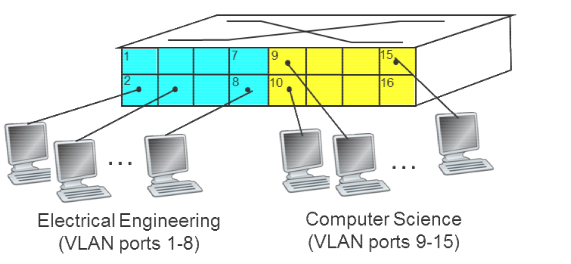
\includegraphics[width=0.7\linewidth]{images/VLAN_1.png}
	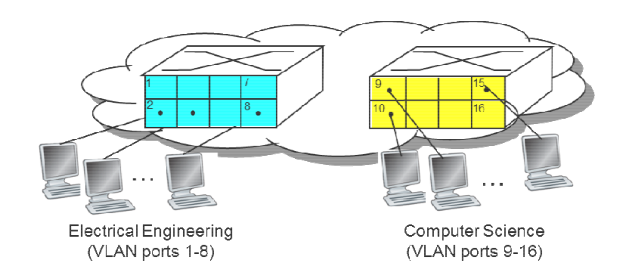
\includegraphics[width=0.8\linewidth]{images/VLAN_2.png}
	\caption{Zusammenfassung der Ports eines Switches zu einzelnen Gruppen \cite[Kapitel 5, Abbildung Folie 41]{netzwerkeI}}
\end{figure}

Jedes Netzwerk verfügt heutzutage über mindestens einen Switch, da mehrere Netzwerkteilnehmer so besser verwaltet werden können.
Früher hat diese Aufgabe ein Hub oder eine Bridge übernommen, bis diese vom Switch abgelöst wurden.
\begin{figure}[H]
	\centering
	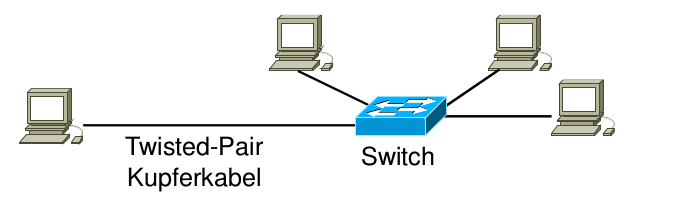
\includegraphics[width=1\linewidth]{images/geswitchtes_netz.png}
	\caption{Geswitchtes Netzwerk \cite[Kapitel 5, Abbildung Folie 33]{netzwerkeI}}
\end{figure}
\subsubsection{Mehrere Switches in einem Netzwerk}
Mehrere Switches in einem Netzwerk sind natürlich möglich, allerdings kann man diese nicht einfach so miteinander verbinden, sonst entsteht eine Schleife.
Ist eine Schleife in einem Netzwerk gelegt, bricht der gesamte Datenverkehr zusammen.

Für die Umsetzung mehrerer Switches in einem Netz müssen ein paar Vorkehrungen getroffen werden, unter anderem spezielle Kabel, um eben diese Schleife zu verhindern.



